\section{Quality aware network (QAN)}

In our work we focus on improving image set embedding model, which maps an image set $S=\{I_1, I_2, \cdots, I_N\}$ to an representation with fixed dimension so that image sets with different number of images are comparable with each other. Let $R_a(S)$ and $R_{I_i}$ denote representation of $S$ and $I_i$. $R_a(S)$ is determined by all elements in $S$, therefore it can be denoted as
\begin{equation}
\small
\label{3}
R_a(S) = \mathcal{F}(R_{I_1}, R_{I_2}, \cdots, R_{I_N}).
\end{equation}

The $R_{I_i}$ is produced by a feature extraction process, containing  traditional hand-craft feature extractors or convolutional neural network.  $\mathcal{F}(\cdot)$ is an aggregative function, which maps a variable-length input set to a representation of fixed dimension. The challenge is to find an optimized $\mathcal{F}(\cdot)$, which aggregate features from the whole image set to obtain the most discriminative representation. 
Based on notion that images with higher quality are easier for recognition while images with lower quality containing occlusion and large pose have less effect on set representation, we denote $\mathcal{F}(\cdot)$ as
\begin{equation}
\small
\label{5}
\mathcal{F}(R_{I_1}, R_{I_2}, \cdots, R_{I_N}) =\frac{\sum_{i=1}^N\mu_i R_{I_i}}{\sum_{i=1}^N\mu_i }
\end{equation}
\begin{equation}
\small
\label{6}
\mu_i = Q(I_i),
\end{equation}
where $Q(I_i)$ predicts a quality score $\mu_i$ for image $I_i$. So the representation of a set is a fusion of each images' features, weighted by their quality scores.

\subsection{QAN for image set embedding}
In this paper, feature generation and aggregation module is implemented through an end-to-end convolutional neural network named QAN as shown in Fig.~\ref{figure_train}. Two branches are splited from the middle of it. In the first branch, quality generation part followed by a set pooling unit composes the aggregation module. And in the second branch, feature generation part  generates images' representation. Now we introduce how an image set flows through QAN. At the beginning of the process, all images are sent into a fully convolutional network to generate middle representations. After that,
QAN is divided into two branches. The first one (upper) named quality generation part is a tiny convolution neural network (see Sec.~\ref{details_qgp} for details) which is employed to predict quality score $\mu$. The second one (lower), called feature generation part,  generates image representations $R_I$ for all images. $\mu$ and $R_I$ are aggregated at set pooling unit $\mathcal{F}$, and then pass through a fully connected layer to get the final representation $R_a(S)$. To sum up, this structure generates quality scores for images, uses these quality scores to weight images' representations and sums them up to produce the final set's representation.

\subsection{Training QAN without quality supervision}
\label{end2endtrain}
We train the QAN in an end-to-end manner. The data flow is shown in Fig.~\ref{figure_train}. QAN is supposed to generate discriminative representations for images and sets belonging to different identities. For image level training, a fully connection layer is established after feature generation part, which is supervised by Softmax loss $L_{class}$. For set level training, a set's representation $R_a(S)$ is supervised by $L_{veri}$ which is formulated as:
\begin{equation}
\small
\begin{aligned}
\label{7}
L_{veri} = &\left \lVert R_a(S_a)-R_a(S_p) \right \rVert^2 - &\left \lVert R_a(S_a)- R_a(S_n) \right \rVert^2 + \delta
\end{aligned}
\end{equation}


The loss function above is referred as \emph{Triplet Loss} in previous works \cite{schroff2015facenet}. We define $S_a$ as \emph{anchor set}, $S_p$ as \emph{positive set}, and $S_n$ as \emph{negative set}.  This function minimizes variances of intra-class samples while Softmax loss cannot guarantee that because softmax-loss directly optimizes the probability of each class, but not the discrimination of representation.


%\begin{equation}
%\footnotesize
%\label{difftrip}
%\begin{split}
%\frac{\partial L_{veri}}{\partial R_a(S_a)} = 2 \cdot (R_a(S_n)- R_a(S_p))  \\
%\frac{\partial L_{veri}}{\partial R_a(S_p)} = 2 \cdot (R_a(S_p)- R_a(S_a))  \\
%\frac{\partial L_{veri}}{\partial R_a(S_n)} = -2 \cdot (R_a(S_a)- R_a(S_n))
%\end{split}
%\end{equation}

% The gradient of Triplet loss tend to push the representations of different people further away while reducing the distance between representations of the same person.

Keeping this in mind, we consider the set pooling operation $\mathcal{F}$. The gradients back propagated through set pooling unit can be formulated as follows,
\begin{equation}
\small
\label{eq9}
\frac{\partial \mathcal{F}}{\partial R_{I_i}} =\frac{\partial R_a(S)}{\partial R_{I_i}} =\mu_i
\end{equation}
\begin{equation}
\small
\label{10}
\frac{\partial \mathcal{F}}{\partial \mu_i} =\frac{\partial R_a(S)}{\partial \mu_i} = R_{I_i} - R_a(S)
\end{equation}
So we can formulate propagation process of the final loss as
\begin{equation}
\small
\begin{aligned}
\label{11a}
\frac{\partial L_{veri}}{\partial R_{I_i}}
&= \frac{\partial R_a(S)}{\partial R_{I_i}} \cdot \frac{\partial L_{veri}}{\partial R_a(S)}  
&= \frac{\partial L_{veri}}{\partial R_a(S)} \cdot \mu_i
\end{aligned}
\end{equation}
\begin{equation}
\small
\begin{aligned}
\frac{\partial L_{veri}}{\partial \mu_i} &= \frac{\partial R_a(S)}{\partial \mu_i} \cdot (\frac{\partial L_{veri}}{\partial R_a(S)})^T  \\
&= \sum_{j=1}^D ( \frac{\partial L_{veri}}{\partial R_a(S)_j} \cdot ( x_{ij} - R_a(S)_j ) )
\label{11b}
\end{aligned}
\end{equation}
Where $D$ is the dimension of images' representation. We discuss how a quality score $\mu$ is automatically learned by this back propagation process.


\subsection{Mechanism for learning quality score}

\begin{figure}[!htbp]
  \centering
  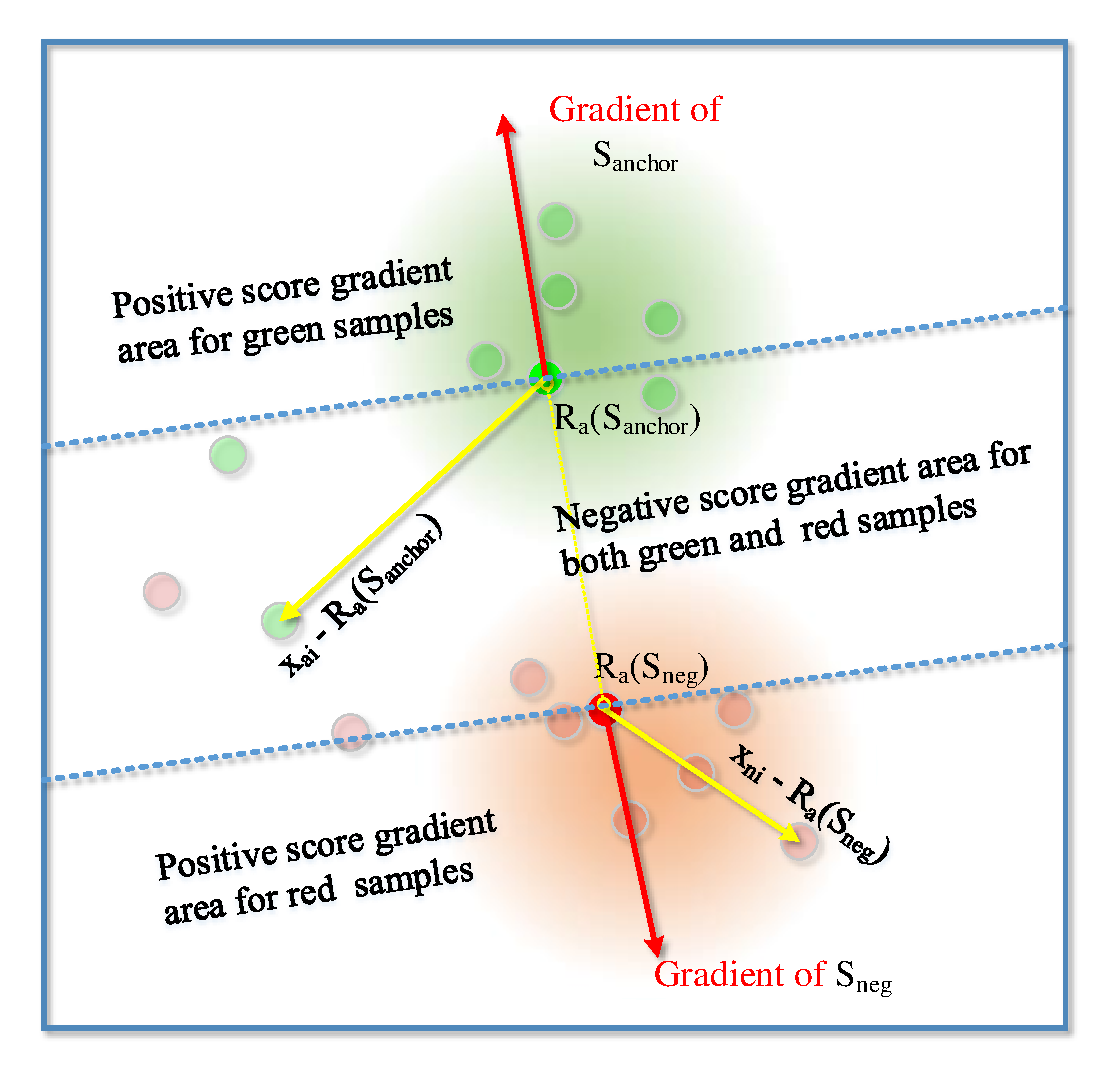
\includegraphics[width=8cm]{figure_gradient.pdf}
  \caption{Two different identities in training, best viewed in color. Red translucent dots and green translucent dots indicate images in sets of two different identities. And the two solid dots denote the weighted centers of the two sets, which are also the representations of two sets $S_{anchor}$ and  $S_{neg}$. The gradients of $S_{anchor}$ and  $S_{neg}$ are shown with red arrows. The $x_{ni}$ and $x_{ai}$ are two image representations in two sets.} 
  \label{fig:gradient}
\end{figure}

\textbf{Automatic gradient of $\mathbf{\mu}$.}
After back-propagation through set pooling unit, gradient of $\mu_i$ with regard to $L_{veri}$ can be calculated according to the Eq.~\ref{11b}, which is the dot product of gradient from $R_a(S)$ and $R_{I_i}$. So if angle of $\nabla R_a(S)$ and $R_{I_i}$ belongs to ($-90^{\circ}$, $90^{\circ}$), $\mu_i$'s gradient will be positive. For example, as shown in Fig.~\ref{fig:gradient}, the angle of $\nabla R_a(S_{neg})$ and $x_{ni}-R_a(S_{neg})$ is less than $90^{\circ}$, so the $x_{ni}'s$ quality score $\mu_{ni}$ will become larger after this back propagation process. In contrast, the relative direction of $x_ai$ is in the opposite side of the gradient of $R_a(S_{anchor})$, making it obviously a hard sample, so its quality score $\mu_{ai}$ will tend to be smaller. Obviously, samples in the ``correct'' directions along with set gradient  always score higher in quality, while those in the ``wrong'' directions gain lower weight. For example in Fig.~\ref{fig:gradient}, green samples in the upper area and red samples in the lower area keep improving their quality consistently while in the middle area, sample's quality reduces. To this end, $\mu_i$ represents whether $i-th$ image is a good sample or a hard sample. This conclusion will be further demonstrated by experiments.

\textbf{$\mathbf{\mu}$ regulates the attention of $R_{I_i}$.}
The gradient of $R_{I_i}$ is shown in Eq.~\ref{11a} with a factor  $\mu_i$, together with the gradient propagated from Softmax loss. Since most of hard samples with lower $\mu_i$ are always poor images or even full of background noises, the factor $\mu_i$ in gradient of  $R_{I_i}$ weaken their harmful effect on the whole model. That is, their impact on parameters in feature generation part is negligible during back propagation. This mechanism helps feature generation part to focus on good samples and neglect ones, which benefits set-to-set recognition.

%\subsection{Adaptive cascade QAN}

%Quality generation part is implemented through a adaptive cascade structure. Similarity with Adaboost\cite{freund1996experiments}, we hope to adapt samples with different quality to the matched quality generation unit.  To implement this, $n$ ($n=2$ in human re-identification task while in face verification task, $n=3$) quality generation units $Q_i,(i=1 to N)$ are established in cascade quality generation part. Each of them contains a threshold $\sigma_i$. The set is regarded as having poor quality in stage $k$ if its average score is lower than $\sigma_k$. Sets with poor $k^{th}$ quality is sent to $k+1$-th quality generation unit for re-evaluation. 

%\begin{figure*}[!htbp]
%  \centering
%  \includegraphics[height=4cm]{c4_algorithm/figure2.pdf}
%  \caption{Structure of quality generation unit. The input of this unit is middle representations of a set which contains N images and it produces the normalized weights of all N images.}
%\label{figure2}
%\end{figure*}

%Each $Q_i$ is a small convolutional neural network with an appropriate number of convolution and downsample layers to fit the input's spatial scale, followed by a fully connected layer to get quality scores. The outputs of this unit are raw quality scale of all elements. Then we use sigmoid and L1-normalization to normalize all raw quality to $\mu_i$. After that, set pooling unit aggregates all features with their weights according to Eq.~\ref{5}.




%We divide the training procedure into three steps.


%As show in Algorithm~\ref{alg:train}, training procedure are split into three steps.


%\begin{algorithm}
%	\caption{Adaptive Cascade QAN with Joint Training}
%	\label{alg:train}
%	\begin{algorithmic}[1]
%		\Require Training Set $\{T\} $ with label $\{L\}$
%		\State $Basemodel = Optimize(\{T\}, \{L\})$\Comment{pre-train feature generation part}
%		\State $\{\hat{T}\} = \{T\}, \{\hat{L}\} = \{L\}$
%		\State Generate $\bf{R}$ \Comment{generate all representations}
%		\For  {$i=1$ to $cascade.number$} \Comment{pre-train $Q$}
%		\State $Q_i = Optimize(\bf{R}, \{\hat{L_i}\})$\Comment{pre-train $Q_i$}
%		\State $\{\mu\} = Q_i(\bf{R})$ \Comment{generate all quality scores}
%		\State $\sigma_i = threshold(90\% of \{mu\}>=\sigma_i)$
%		\State $\{\hat{T_i}, \hat{L_i}\} = \{\hat{T_i}, \hat{L_i} | \mu_i < \sigma_i\}$\Comment{select poor samples}
%		\EndFor
%		\While{ $iter < maxiter$ } \Comment{joint-train QAN}
%		\State Random select batch samples $\{\hat{T}, \hat{L}\} \in \{T, L\}$
%		\State $Generate \bf{R}$ by $\{\hat{T}\}$
%		\For  {$i=1$ to $cascade.number$}
%		\State $\mu = Q_i(\bf{R})$
%		\If{ $max(\mu)>=\sigma_i $ }
%		\State$\mu=normalize(\mu)$
%		\State break
%		\EndIf
%		\EndFor
%		\State Continue forwarding and back propagating.
%		\EndWhile
%	\end{algorithmic}
%\end{algorithm}
%First, feature generation part is pre-trained with classification signal. And we generate $\{R\}$ for all training data by it.
%After that, the first quality generation unit can be trained with $\{R\}$. This is implemented by fixing all parameters in feature generation part and by only updating parameters in $Q_1$ . After $Q_1$ is pre-trained, we use it to summarize quality scores of all training data and assign $\mu_1$ the borderline of the top 90\% scores. Then all images with quality scores higher than $\mu_1$ are removed from training set and the remaining images are used to train the second quality generation unit $Q_2$. This procedure will loop cascade number times to pre-train all quality generation unit.
%Finally, we jointly train the whole adaptive cascade QAN. During each iteration, final qualities of images in a certain sequence depend on the maximal quality of the sequence. All quality scores of images in this sequence will be generated by a same score generation unit.


%During this procedure, scores of sequence with high-quality images will be generated by former units while those with low-quality will be generated by latter units.

\subsection{Details of quality generation part}
\label{details_qgp}

\begin{figure}[!htbp]
  \centering
  \includegraphics[height=3.1cm]{figure2.pdf}
  \caption{Structure of quality generation unit. The input of this unit is middle representations of a set which contains N images and it produces the normalized weights of all N images.}
  \label{qgu}
\label{figure2}
\end{figure}



\begin{figure*}[!ht]
  \centering
  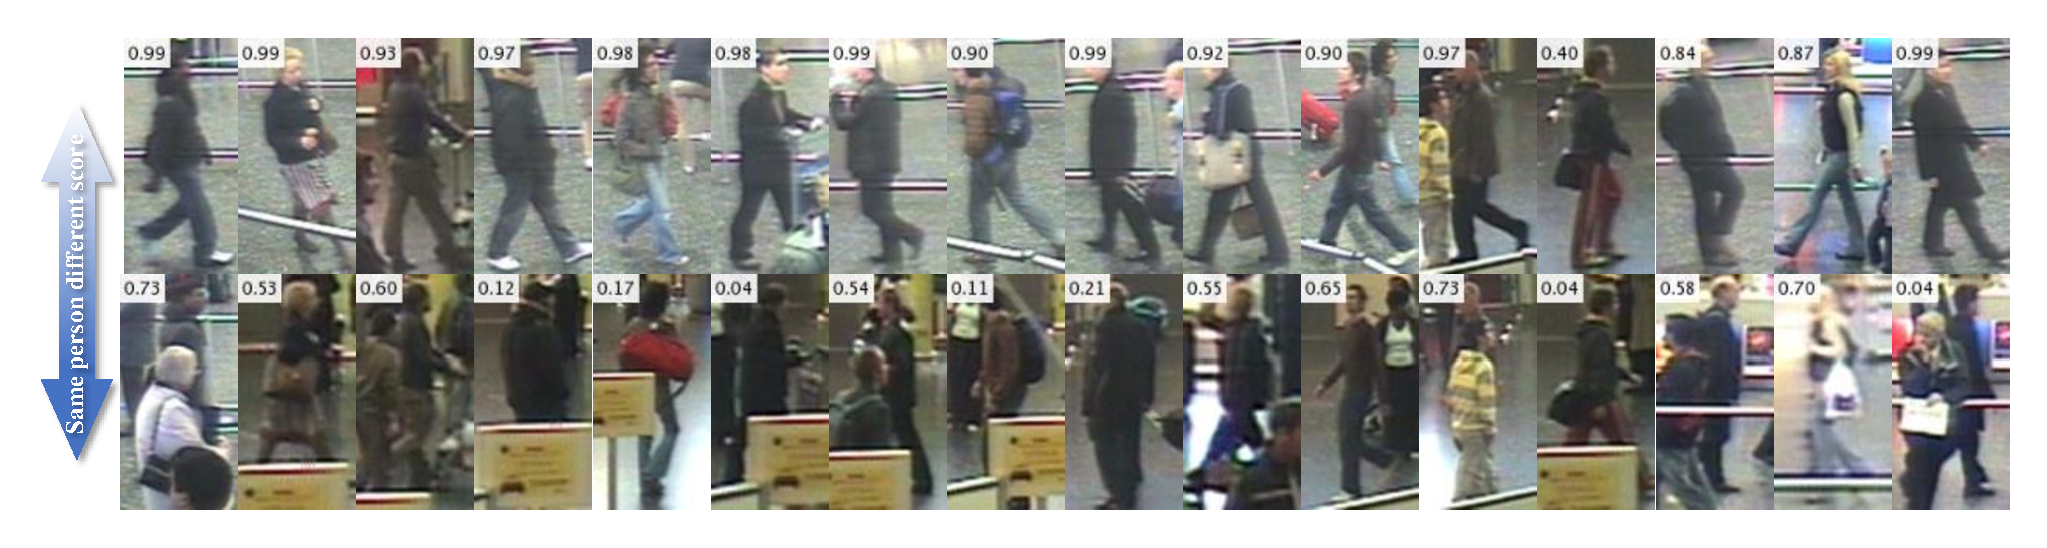
\includegraphics[width=16cm]{supp_sameperson.pdf}
  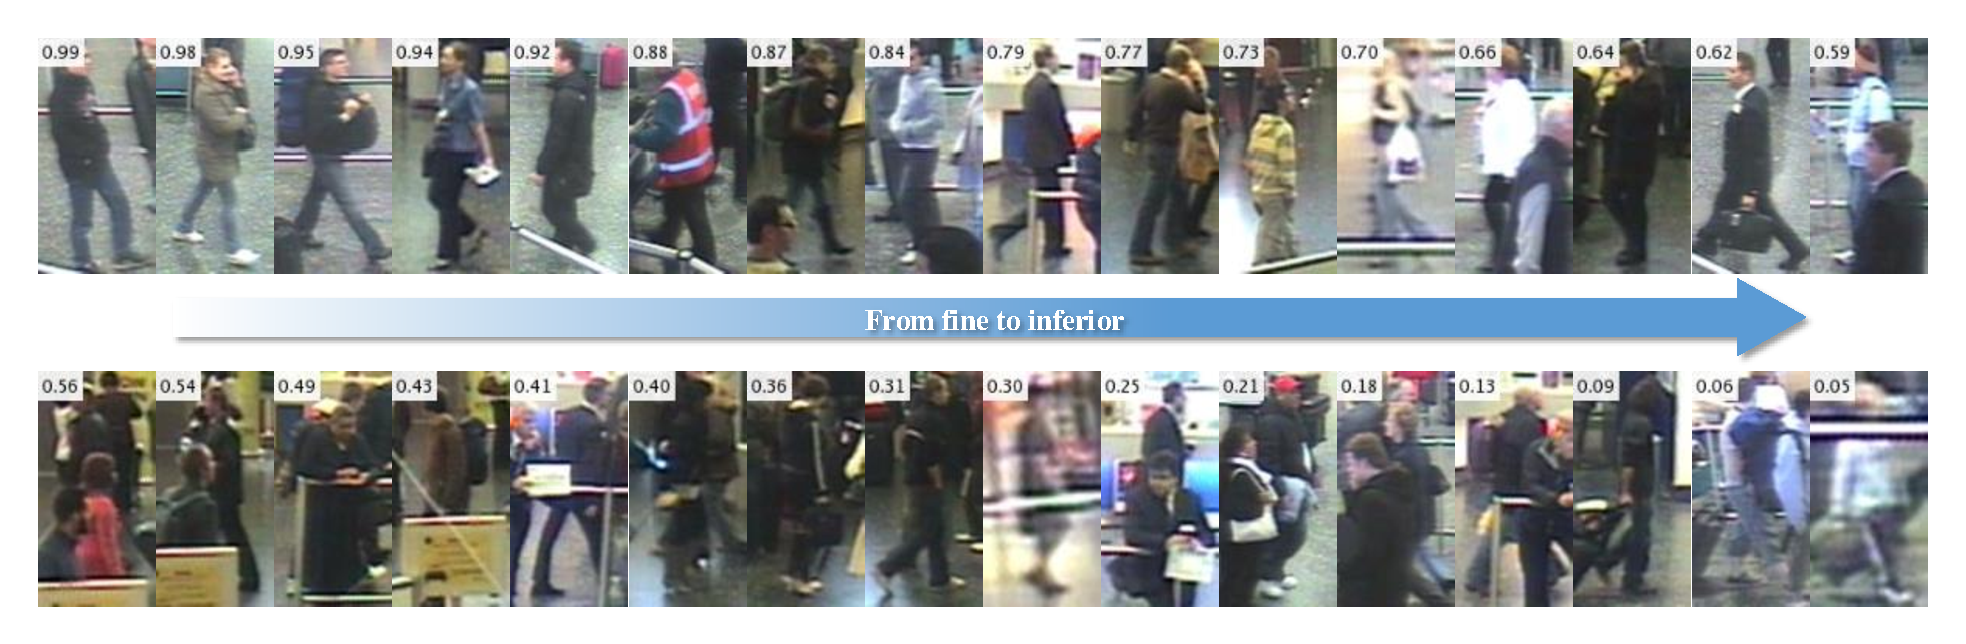
\includegraphics[width=16cm]{supp_sortbyscore.pdf}
  \caption{Samples with their qualities predicted by QAN, best viewed in color. \textbf{Top:} Comparison between two images from same person. From \textbf{up to down}, each column shows the two frames of a same person. The quality of the top one is better than the bottom one. \textbf{Bottom:} Random selected images in test set sorted by quality scores from \textbf{left to right}, best viewed in color.}
  \label{fig:samples}
\end{figure*}

In quality aware network (QAN), quality generation part is a  convolution neural network. We design different score generation parts start at different feature maps. We use QAN split at Pool4 as an instance. As shown in Fig.~\ref{qgu}, the output spatial of Pool4 layer is $512\times14\times14$. In order to generate a $1\times1$ quality score, the convolution part contains a 2-stride pooling layer and a final pooling layer with kernel size $7\times7$. A fully connected layer is followed by the final pooling layer to generate the original quality score. After that, the origin scores of all images in a set are sent to sigmoid layer and group L1-normalization layer to generate the final scores $\mu$. For QAN split at \texttt{Pool3}, we will add a block containing three 1-stride convolution layer and a 2-stride pooling layer at the beginning of quality generation unit.